\documentclass[letterpaper, 12pt]{article}
\usepackage{graphicx}
\graphicspath{{Figures/}{./}}
\usepackage{apacite}
\usepackage{amsmath}
\usepackage{amssymb}
\usepackage{amsthm}
\usepackage{indentfirst}
\usepackage[justification=centering]{caption}
\usepackage{float}

\title{MATHEMATICS ANALYSIS AND APPROACHES HL
\\
Producing the IB Logo with the Fourier Series}
\author{}
\date{}

\begin{document}
\nocite{*}

\maketitle
\begin{center}
    Candidate Code:
    \\
    Session: May 2024
    \\
    Page Count:
\end{center}
\newpage

\tableofcontents
\newpage

\section{Rationale}

I have shown interest in visual arts done through the means of software,
with particular experience in 3D modelling and animation in Blender
and Cinema 4D.

I never was experienced with drawing, therefore producing digital art
on a 2D plane using artistic skill was not of interest to me. However,
something that I came across online was the use of the Fourier Series
in order to produce vector art, which instantly intrigued me.

While vector art files such as those with the file extension ".svg" relate
to mathematics in the sense that it contains multiple graphed mathematical
relationships in order to produce an image, the method of using the Fourier
Series to produce similar art is more mathematically intriguing, as it
proves use just one expression to produce the same result done by the numerous mathematical
relationships.


\section{Aim}

The objective of this investigation is to link Fourier series with
complex numbers to create a single series that is capable
of reproducing the IB logo on the Argand plane.

\section{Plan of Action}

This exploration focuses on the following areas of math:
\begin{itemize}
    \item Integral Calculus
    \item Series
    \item Trigonometry
    \item Complex Analysis
    \item Vectors
\end{itemize}

\section{Background Information}

\subsection{Overarching idea of the Fourier Series}

A periodic function is one where the output for a particular input equals to
the output for the sum of the same input and the value of the function's period.
This can be represented mathematically as:
\begin{align*}
     & f(x) = f(x + P)
    \\
     & \text{where } P = \text{ the period of the function}
\end{align*}

The sine wave is widely known for being a periodic function for the ease of graphing
a sinusoidal wave. However, there are periodic functions that are difficult to
graph with an algebraic expression, such as one that alternates between
1 and -1 or one that is shaped as a zig-zag.

This is the motivation behind the Fourier Series, which is to be able to represent
period functions that normally can't be represented by an algebraic function.

The idea behind the Fourier Series is to take an infinite sum of varying sinusoidal
functions such that a desired periodic function is produced.

\begin{figure}[H]
    \centering
    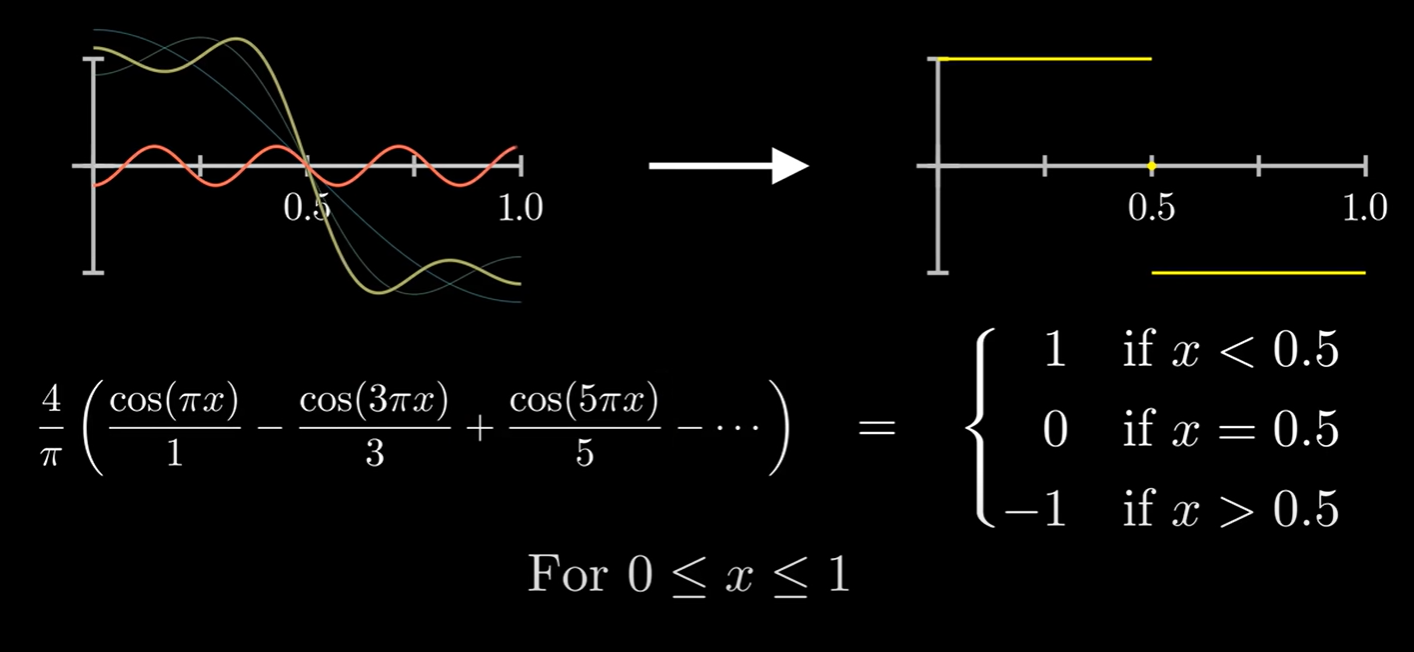
\includegraphics[width=\textwidth]{fourier_basic_visual.png}
    \caption{Visualization of the mechanism of the Fourier Series \protect\cite{sandersonWhatFourierSeries2019}. The yellow line is the periodic function resulting from the previous iteration, the red line is the sinusoidal function to be added in the next iteration.}
    \label{fig:fourier_visual}
\end{figure}

% For reference, a general formula for representing a periodic function as a Fourier Series with a
% period of \(2\pi\) is:
% \begin{equation}
%     f(t) = \frac{a_0}{2} + \sum_{n = 1}^{\infty} a_n \cos{nt} + \sum_{n=1}^{\infty} b_n\sin{nt}
% \end{equation}

% This formula won't be explored in depth, however, it is included as it will
% emphasize how the Fourier Series can be linked with complex numbers.

\subsection{Idea of drawing with the Fourier series explained with the Cartesian Plane}

The rule is for eligible drawings to be any that can be drawn by starting at one point
on a cartesian plane and, without lifting the hypothetical plane throughout the entire
sketch, return to the exact same point.

Defining the variable \(t\) as time, \(t = 0\) will represent the point in time
where the drawing began and \(t = 1\) will represent the point in time where
the drawing ended.

Each point of the drawing on the plane will be defined by \(P(x(t), y(t))\),
where \(x(t)\) and \(y(t)\) are both functions with an input of \(t\) that
indicates the coordinates after some amount of time passed of the pen's progress
through the drawing.

Assuming that any function can be represented as a Fourier Series, then
\(x(t)\) and \(y(t)\) can be any function and therefore, by extracting
the coordinates on a graph of any drawing obeying the rule described earlier,
the Fourier Series of \(x(t)\) and \(y(t)\) can be determined and therefore
produce the desired drawing for \(t\in [0,1]\)
\\

As a simple example that does not require a Fourier Series,
we can take a unit circle defined by \( x^2 + y^2 = 1 \) as the drawing.
It quickly becomes evident of what \(x(t)\) and \(y(t)\) are, as since it is a circle,
then \(x(t) = \cos(2\pi t)\) and \(y(t) = \sin(2\pi t)\).

\subsection{Enriched application to draw on the Argand Plane}

Euler's formula is defined to be
\[
    e^{it} = \cos(t) + i\sin(t)
\]

Given that both the cosine function and the sine function are included in this
formula, a connection between this formula and the Fourier Series becomes evident.
The two sinusoidal functions in the formula are the core behind applying the
Fourier Series to the Argand Plane.

It is easier to think of Euler's formula to be a vector on the Argand Plane\cite{sandersonWhatFourierSeries2019}.
With just the formula given above, we have a vector with a length of 1 that rotates
counterclockwise for larger values of \(t\) and clockwise for smaller values of \(t\).


\begin{align*}
     & f(t) = \sum_{n=-\infty}^{\infty} c_n e^{n \cdot 2\pi it}
    \\
     & c_n = \int_{0}^{1} f(t) e^{-n \cdot 2\pi it} \,dt
\end{align*}


\bibliographystyle{apacite}
\bibliography{IB_MATH_IA.bib}

\end{document}